\documentclass{beamer}

\usepackage[utf8x]{inputenc}
\usepackage{graphicx}
\usepackage{tabularx}
\usepackage[brazil]{babel}
\usetheme{PaloAlto}
\usecolortheme{rose}

\title[Operações Geométricas (Warping) em Imagens]{Operações Geométricas
(Warping) em Imagens}
\author[Roberto Azevedo]{Roberto Gerson de Albuquerque Azevedo}
\institute{Foundations of Computer Graphics 2011.1 PUC-Rio}
\date{\today}
\subject{alguma coisa}
%\logo{\includegraphics[scale=1.0]{sua_figura.png}}

\begin{document}
%para criar a página de rosto
\frame{\titlepage} %inclui a front page 
%==================================================slide
% cria o sumário
\begin{frame}
 \frametitle{Sumário}
 \tableofcontents
\end{frame}
%-------------------------------------------------------
%==================================================slide
\section{Introdução}
\begin{frame}
\frametitle{Introdução}
\begin{itemize}
 \item Operações Geométricas (ou filtros geométricos, ou \textit{Warping}) tem
como objetivo alterar as posições dos pixels da imagem, baseada em alguma função
de mapeamento.
  \item Extremamente útil para o mapeamento de texturas.
  \item Em princípio, uma operação geométrica transforma uma dada imagem $I$
para uma nova imagem $I'$ modificando as coordenadas dos pixels da imagem:
\par
\begin{center}
 $I(x,y) \rightarrow I'(x', y')$
\end{center}

\end{itemize}
\end{frame}

%-------------------------------------------------------
%==================================================slide
\subsection{Exemplos}
\begin{frame}
 \frametitle{Transformações Geométricas - Exemplos}
\begin{figure}[ht!]
  \centering
  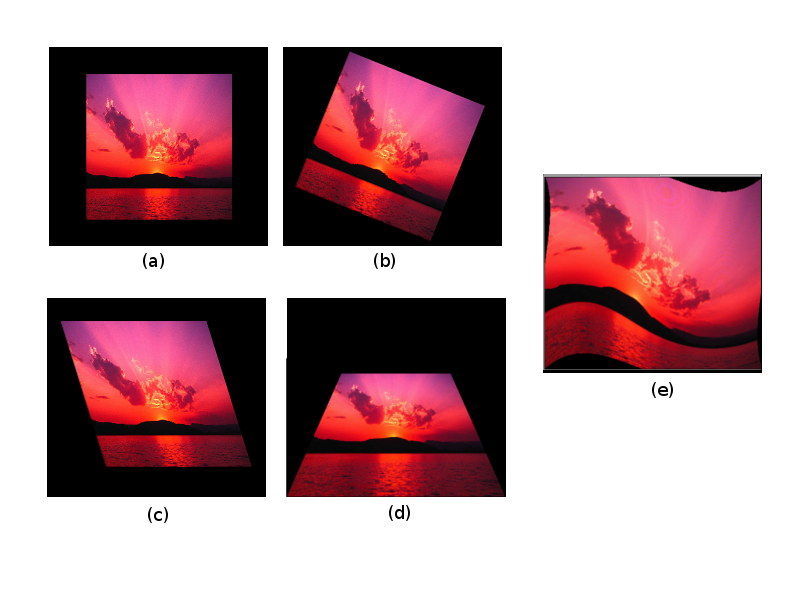
\includegraphics[width=0.75\textwidth]{img/typical-geometric-transform.png}
\end{figure}
Exemplos de transformações geométricas em imagens: (a) escala; (b) rotação; (c)
cisalhamento; (d) perpectiva; e (e) twirl.
\end{frame}

%-------------------------------------------------------
%==================================================slide
\subsection{Classificação}
\begin{frame}
 \frametitle{Transformações Geométricas - Classificação}
\begin{figure}[ht!]
  \centering
  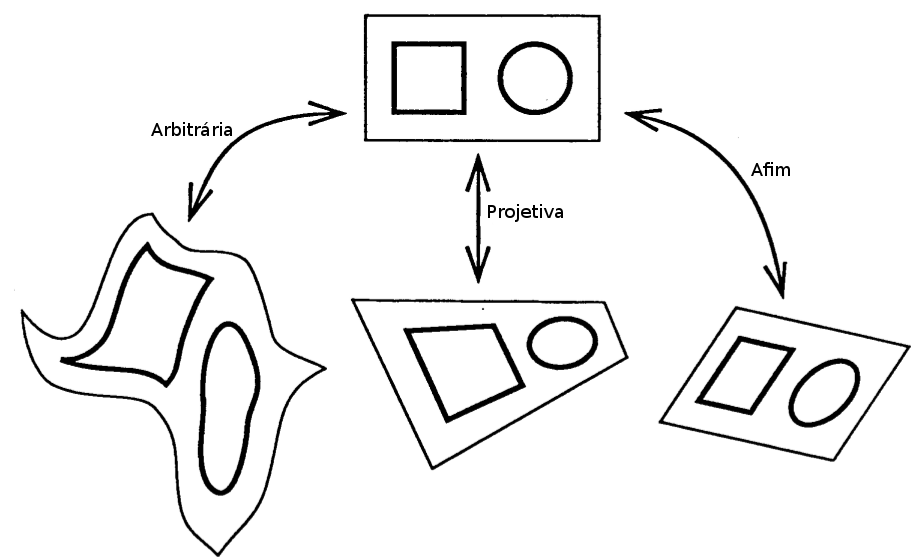
\includegraphics[width=0.75\textwidth]{img/affine-projective-arbitrary.png}
\end{figure}
\end{frame}

%-------------------------------------------------------
%==================================================slide
\section{Função de Mapeamento}
\begin{frame}
\frametitle{Reamostragem: Source-to-target X Target-to-source}
\begin{tabular*}{0.75\textwidth}{ p{4cm} p{.6cm} p{4cm}}
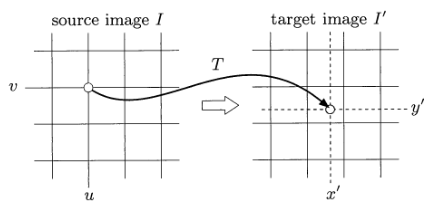
\includegraphics[width=1.9in]{img/source-to-target-mapping.png}  & &
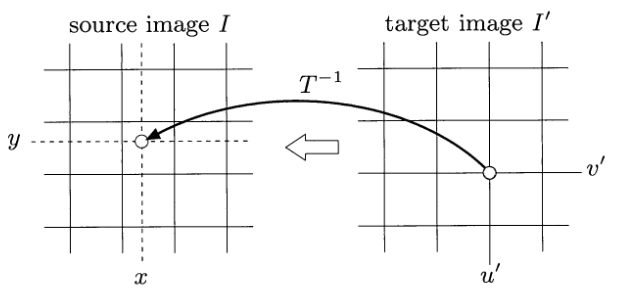
\includegraphics[width=1.9in]{img/target-to-source-mapping.png} \\
\scriptsize
\textbf{Source-to-target}: Para cada pixel $(x,y)$ da imagem original
$I$ a posição transformada em $I'$ é dada por: 
\begin{equation*}
 (u,v)=T(x,y)
\end{equation*} & &
\scriptsize
\textbf{Target-to-source}: Para cada pixel $(u',v')$ da imagem final
$I'$, é computado o ponto correspondente (contínuo) da imagem original: 
\begin{equation*}
 (x, y)=T^{-1}(u',v')
\end{equation*} \\
\end{tabular*}
\end{frame}

%-------------------------------------------------------
%==================================================slide
\subsection{Problemas na Reamostragem}
\begin{frame}
\frametitle{Transformações Geométricas - Problemas}
\begin{itemize}
 \item Operações geométricas não são simples, porque envolvem reamostrar os
pixels que inicialmente são discretos em um domínio de reais.
 \item Problemas:
 \begin{itemize}
  \item Magnificação - duplica informação (serrilhado)
  \item Minimificação - perde informação (\textit{aliasing})
 \end{itemize}
\end{itemize}
\begin{figure}[ht!]
  \centering
  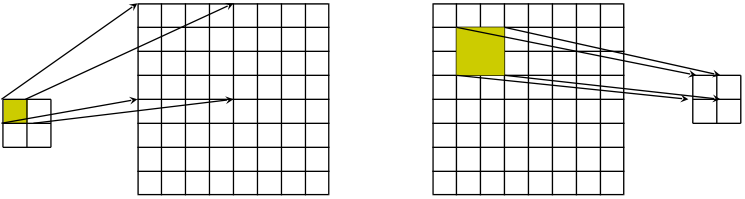
\includegraphics[width=0.8\textwidth]{img/resize.png}
\end{figure}
\end{frame}
%-------------------------------------------------------
%==================================================slide
\begin{frame}
  \frametitle{Reamostragem: Interpolação}
\begin{itemize}
 \item A função de mapeamento comumente é uma função $R^2 \rightarrow R^2$.
 \item Como tanto a imagem original como a imagem final são discretas, quase
sempre temos um problema de reamostragem depois de aplicar a função de
mapeamento.
\end{itemize}
\begin{center}
 \framebox{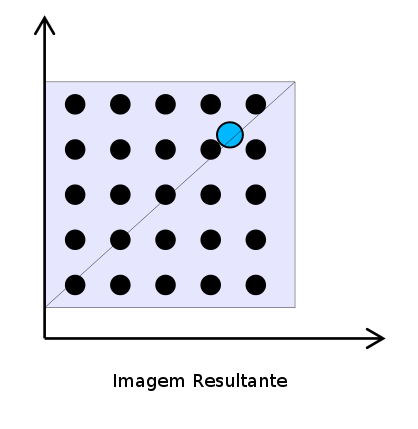
\includegraphics[width=1.2in]{img/pixels-in-resulting-image.png}}
\end{center}
\end{frame}

\begin{frame}
  \frametitle{Reamostragem: "Interpolação" (Nearest Neighbor)}
\begin{itemize}
 \item A função de mapeamento comumente é uma função $R^2 \rightarrow R^2$.
 \item Como tanto a imagem original como a imagem final são discretas, quase
sempre temos um problema de reamostragem depois de aplicar a função de
mapeamento.
\end{itemize}
\begin{center}
 \framebox{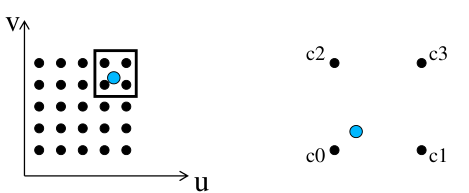
\includegraphics[width=2.5in]{img/nearest-neighbor.png}}
\end{center}
\end{frame}

%-------------------------------------------------------
%==================================================slide
\subsection{Twirl}
\begin{frame}
\frametitle{Twirl}
\begin{itemize}
 \item A transformação "Twirl" faz uma rotação na imagem ao redor de um dado
ponto $p_c = (x_c, y_c)$ com variação espacial em relação ao ângulo de rotação
$\alpha$.
 \item A imagem se mantém inalterada fora de um limite dado por $r_{max}$.
\end{itemize}

\begin{columns}[c]
\column{1.5in}
\textbf{Input:} \\
Centro: $p_c = (x_c, y_c)$ \\
Ângulo de Rotação: $\alpha$ \\
Raio Máximo: $r_{max}$ 
\column{1.5in}
\framebox{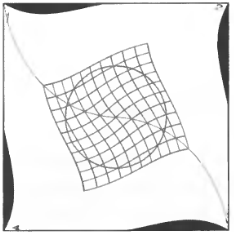
\includegraphics[width=1.5in]{img/twirl.png}}
\end{columns}
\end{frame}

%-------------------------------------------------------
%==================================================slide
\begin{frame}
\frametitle{Twirl: Função de Mapeamento Inverso}
A Função de Mapeamento inverso da transformação \textit{twirl} (dado um ponto da
textura $(u,v)$, determina o ponto correspondente na image) é dada por:

   \begin{equation}
    T_x^{-1}: x = 
\begin{cases}
 x_c + r.cos(\beta), & \text{se } r \leq r_{max}\\
 x', & \text{se } r > r_{max}
\end{cases}
   \end{equation}

\begin{equation}
    T_y^{-1}: y = 
\begin{cases}
 y_c + r.sin(\beta), & \text{se } r \leq r_{max} \\
 y', & \text{se } r > r_{max}
\end{cases}
\end{equation}

Onde,
\begin{equation}
\begin{array}{c|c}
d_x = x'- x_c & r = \sqrt[2]{d_x^2+d_y^2} \\
d_y =  y'- y_c & \beta = AcTang(s_x, d_y + \alpha.(\frac{r_max-r}{r_max}))
\end{array}
\end{equation}
\end{frame}

%-------------------------------------------------------
%==================================================slide
\subsection{Spherical}
\begin{frame}
 \frametitle{Spherical}
\begin{itemize}
 \item A deformação esférica imita o efeito de visualizar uma imagem por meio
de uma meia esfera ou lente posta sobre a imagem.
\end{itemize}
 
\begin{columns}[c]
\column{1.5in}
\textbf{Input:} \\
Centro da lente esférica: $p_c = (x_c, y_c)$ \\
Raio da lente: $r_{max}$ \\
Índice de refração: $\rho$
\column{1.5in}
\framebox{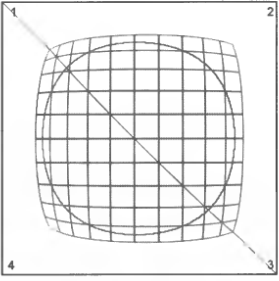
\includegraphics[width=1.5in]{img/sphere.png}}
\end{columns}
\end{frame}

\begin{frame}
 \frametitle{Spherical: Função de mapeamento inverso.}
  \begin{equation}
    T_x^{-1}: x = x' -
\begin{cases}
 z.tan(\beta_x), & \text{se } r \leq r_{max}\\
 0, & \text{se } r > r_{max}
\end{cases}
   \end{equation}

\begin{equation}
    T_y^{-1}: y = y' - 
\begin{cases}
 z.tan(\beta_y), & \text{se } r \leq r_{max} \\
 0, & \text{se } r > r_{max}
\end{cases}
\end{equation}

Onde,
\begin{equation}
\begin{array}{c|c|c}
d_x = x'- x_c & r = \sqrt[2]{d_x^2+d_y^2}  & \beta_x =
(1-\frac{1}{\rho}.sin^-1(\frac{d_x}{\sqrt[2]{d_x^2+z^2}}))\\
 & & \\
d_y =  y'- y_c & z = \sqrt[2]{r_max^2 - r^2} & \beta_y = 
(1-\frac{1}{\rho}.sin^-1(\frac{d_x}{\sqrt[2]{d_y^2+z^2}}))
\end{array}
\end{equation}
\end{frame}

%-------------------------------------------------------
%==================================================slide
\subsection{Perspective}
\begin{frame}
 \frametitle{Perspective}
 \begin{itemize}
  \item A projeção perspectiva é uma transformação linear entre quadriláteros
arbitrários.
  \item A projeção perspectiva pode ser escrita como um mapeamento linear em
coordenadas homogêneas:
 \end{itemize}

\begin{columns}[c]
\column{1.5in}
%\[
% \begin{bmatrix}
%      x' & y' & h'
%  \end{bmatrix} 
%  = 
%  \begin{bmatrix} x & y & 1 \end{bmatrix} . 
%\begin{bmatrix} 
%  a_{11}
%\end{bmatrix}
%\]
\column{1.5in}
\framebox{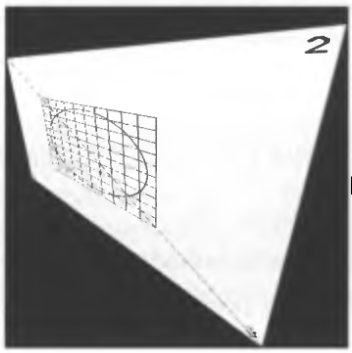
\includegraphics[width=1.5in]{img/perspective.png}}
\end{columns}

\end{frame}

%-------------------------------------------------------
%==================================================slide
\begin{frame}
 \begin{itemize}
  \item TODO: EWA.
  \item TODO: Enhanced EWA.
 \end{itemize}
\end{frame}

%\section{Filtros}
%\subsection{Linear}
%\subsection{Billinear}

%\subsection{EWA - Elliptical Weighted Average Filter}
%\begin{frame}
%\frametitle{Ellipitcal Weighted Average Filter}
%\begin{itemize}
% \item 
%\end{itemize}
%\end{frame}

%-------------------------------------------------------
%==================================================slide
\begin{frame}
\frametitle{Conclusões}
\begin{itemize}
 \item Transformações geométricas não são simples.
 \item Filtros são necessários.
 \item Filtros isotrópicos / anisotrópicos.
\end{itemize}
\end{frame}

\end{document}
